% \section{Jste u nás poprvé?}

% \bigskip
% \subsection{Půjčovna}

% \bigskip
\ifdefined\ikonka\else%
\newcommand\ikonka[1]{\bigskip\bgroup\Large #1\egroup\par}
% \newcommand\ikonka[1]{}
\renewcommand\section[2][]{%
  \bgroup\large \textbf{#2}\egroup\par%
}
\fi
\ikonka{\faPencil}
\section{Vyplňte přihlášku online}

%Její vyplnění je zdarma. 
Vyzvedněte si průkaz UK v \href{http://www.cuni.cz/UK-3249.html}{\emph{Informačním a poradenském
centru UK}}. 
% \textit{\url{knihovna.cuni.cz/e-prihlaska/}}.
Díky tomuto průkazu se můžete zdarma přihlásit do všech knihoven UK přes následující odkaz:

\qrodkaz{knihovna.cuni.cz/e-prihlaska/}

\ikonka{\faSearch}
\section{Vše najdete ve vyhledávači UKAŽ}
% \url{ukaz.cuni.cz}

\vspace{-1em}
\begin{enumerate}
  \item Čtenářské konto (přehled výpůjček, možnost jejich prodloužení).

  \item Veškeré tištěné zdroje. Vyhledejte signaturu požadované knihy (např. F54759) a předejte ji u pultu knihovníkům.

  \item Veškeré elektronické zdroje dostupné na UK (e-knihy, e-časopisy, e-články).\\ Jejich přehled najdete zde \textit{knihovna.pedf.cuni.cz/eiz.htm}.
\end{enumerate}

\vspace{-1em}
\ikonka{\faBook}
\section{Půjčování a vracení }

Většinu knih máme ve skladu, ale připravujeme je obratem.

Knihy můžeme nachystat i předem a umístit je do výdejního boxu před studovnou.
Bez ohledu na naši otevírací dobu si je můžete vyzvednout. Kód k vyzvednutí
zasíláme SMS zprávou.

Standardní výpůjční lhůta je 30 dní a je možné ji prodloužit. 
K vracení knih
můžete využít výpůjční pult, nebo bibliobox -- jeden u vrátnice v M. Rettigové 4 a jeden před
studovnou v Celetné 13. Do biblioboxů vkládejte jen knihy půjčené na dané pobočce.




\ikonka{\faBed}
\section{Studujte pohodlně z domova}
Kromě papírových knih a časopisů máme i
stovky tisíc textů elektronicky.  V~nabídce jsou elektronické
časopisy, články nebo knihy různých oborů. 

Více informací naleznete např. na~\textbf{Portálu elektronických zdrojů
  {\href{https://ezdroje.cuni.cz}{Univerzity Karlovy}}} nebo ve \textbf{vyhledávači UKAŽ}.

\ikonka{\faAndroid}
\section{Pomoc s citacemi}

Pokud studujete nebo pracujete na Pedagogické fakultě, můžete bezplatně
využívat citační manažer Citace PRO. 

\qrodkaz{www.citacepro.com/}

% Pokud si s citacemi nevíte rady, rádi pomůžeme.
% Tvořit citace je jednoduché: nechte za sebe pracovat citační manažer.
% Pokud studujete nebo pracujete na~Pedagogické fakultě,
% můžete bezplatně využívat citační manažer Citace PRO.
% Pokud si s citacemi nevíte rady, rádi pomůžeme.

% \newpage

\ikonka{\faInfoCircle}
\section{Poradíme on-line i osobně} 
% Na dálku poradíme s citováním i rešeršemi přes FB knihovny.

Zajímá vás, jak ke zvolenému tématu efektivně vyhledat informace, pracovat se
zdroji nebo jak správně citovat? Poradíme vám přes Instagram, FB, e-mail, ale
můžeme si také domluvit osobní konzultace v knihovně.
% Zajímá vás, jak efektivně vyhledávat informace, pracovat se zdroji nebo jak
% správně citovat? Ptejte se v naší online poradně přes FB @knihovnapedfpraha,
% nebo nám napište na e-mail. Můžeme si také domluvit osobní konzultace. 


% \newpage

\ikonka{\faGraduationCap}
\section{Vyzkoušejte naše studovny}

Kromě knih a časopisů tu najdete počítače, tiskárny, kopírky a
skener. Nabízíme také vázání \textbf{kroužkovou vazbou}. 
% Půjčujeme i notebooky, USB
% nabíječky na telefon, čtečky elektronických knih, deskové hry nebo flash disky. 

% Pro prezenční studium dokumentů je určena studovna knihovny. 
% Tu mohou využívat studenti s~platným průkazem UK, ale i externí uživatelé. 
% Uloženy jsou zde 
% Ve studovně najdete odborné knihy, odborné i populárně naučné
% časopisy, učebnice, skripta a vždy aktuální denní tisk.

% Využít můžete počítače s přístupem na~internet a do databází,
% samoobslužné tiskárny, kopírky a skener. Nabízíme také vázání kroužkovou vazbou.

% Můžete využít i doplňkových služeb a vypůjčit si 
% Půjčujeme i notebooky, USB nabíječky na
% telefon, čtečky elektronických knih, deskové hry nebo flash disky (vše
% v~rámci studovny).

% \textbf{Máme pro vás týmovou studovnu.} Rezervovat si ji můžete
% vyplněním formuláře na~našem webu. V týmové studovně je k dispozici deset míst
% a tabule na~psaní.
\textbf{Máme pro vás týmovou studovnu},  kde je k dispozici deset míst, deskové hry
a tabule na~psaní.

% \subsection{Další služby a nástroje}

% \newpage



\bigskip
\ikonka{\faHeart}
\section{Služby pro studující se~speciálními potřebami}

Studovna je vybavena počítačem se screen readerem NVDA a s Fine readerem.
Můžete využít bezplatný tisk materiálů souvisejících se studiem a
bezplatné obalování knih. K dispozici jsou také digitalizované knihy přístupné prostřednictvím Centra Carolina.


% Studovna je vybavena počítačem s nainstalovaným screen readerem NVDA a Fine
% Readerem. Tento počítač je volně dostupný a je možné ho využívat samostatně.
% Pro studenty se zrakovým znevýhodněním je k dispozici 245 zdigitalizovaných
% knih. Přístupné jsou z webu knihovny. Na základě registrace obdržíte heslo pro
% online přístup k nim. Tato registrace umožňuje také bezplatný tisk materiálů
% souvisejících se studiem. Pro individuální přístup s ohledem k Vašim
% specifickým potřebám nás neváhejte kontaktovat.  

\vfill

\begin{center}
 
\includegraphics[width=0.5\textwidth]{knihy.png}
\end{center}

\newpage
\section{Kde nás najdete?}

\vskip 1em
\smallsection{Půjčovna a studovna v hlavní budově fakulty}

% Těšíme se na~vás v přízemí hlavní budovy Pedagogické fakulty
% na~adrese 
Magdalény Rettigové 4, Praha 1\\
v přízemí.

% \vskip 3em

\includegraphics[width=\textwidth]{mapka-texty.png}

\vskip 1em
\smallsection{Studovna v Celetné}

Celetná 13, Praha 1, v podkroví

\begin{center}

\includegraphics[width=0.4\textwidth]{schody.png}
\end{center}


% \textbf{Jak se k~nám dostanete?}

% \begin{itemize}[leftmargin=0pt, topsep=0pt]
% \item
%   metrem B, stanice Národní třída -- výtahem přímo do ulice Magdalény
%   Rettigové
% \item
%   tramvají č. 3, 6, 9, 14, 24 zastávka Lazarská
% \end{itemize}

% \smallsection{Knihovna je rozdělena na dvě části:}

% \begin{itemize}[leftmargin=0pt, topsep=0pt]
% \item Půjčovna se nachází napravo od hlavního vchodu
%   do budovy, přes dvorek, vedle zadního vchodu do Auly.
% \item Studovna  je na levé straně budovy.
% \end{itemize}

  % \rotatebox{90}{% Graphic for TeX using PGF
% Title: /home/mint/knihovna/planekknihovny.dia
% Creator: Dia v0.97.3
% CreationDate: Tue Oct 10 14:49:24 2017
% For: mint
% \usepackage{tikz}
% The following commands are not supported in PSTricks at present
% We define them conditionally, so when they are implemented,
% this pgf file will use them.
\ifx\du\undefined
  \newlength{\du}
\fi
\setlength{\du}{11\unitlength}
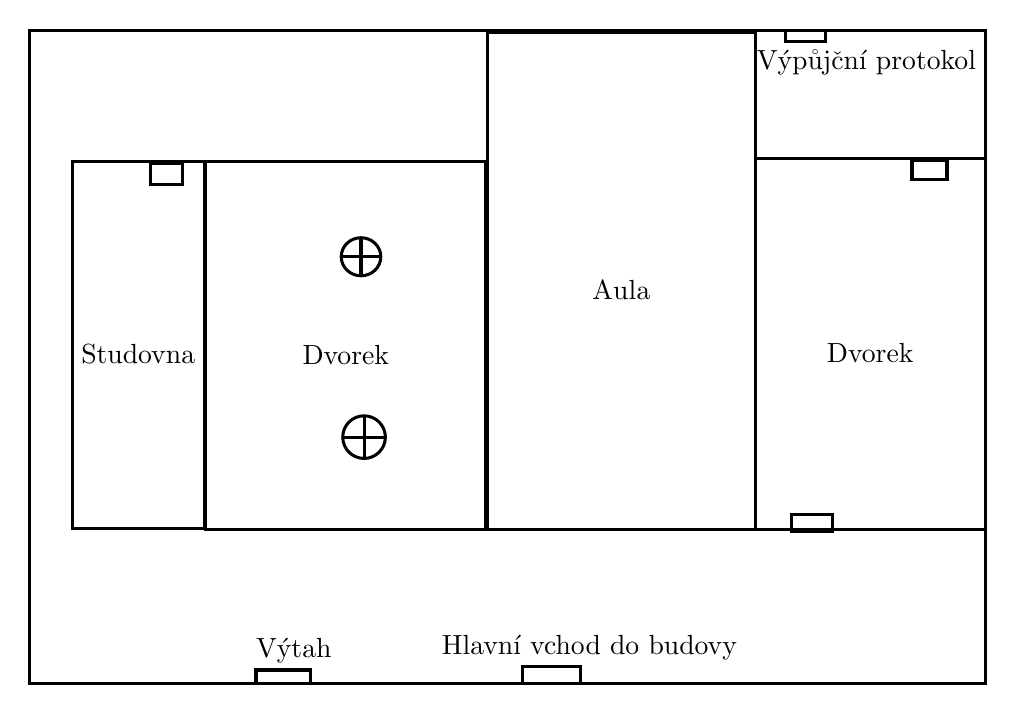
\begin{tikzpicture}
\pgftransformxscale{1.000000}
\pgftransformyscale{-1.000000}
\definecolor{dialinecolor}{rgb}{0.000000, 0.000000, 0.000000}
\pgfsetstrokecolor{dialinecolor}
\definecolor{dialinecolor}{rgb}{1.000000, 1.000000, 1.000000}
\pgfsetfillcolor{dialinecolor}
\definecolor{dialinecolor}{rgb}{1.000000, 1.000000, 1.000000}
\pgfsetfillcolor{dialinecolor}
\fill (0.300000\du,4.300000\du)--(0.300000\du,25.750000\du)--(31.700000\du,25.750000\du)--(31.700000\du,4.300000\du)--cycle;
\pgfsetlinewidth{0.100000\du}
\pgfsetdash{}{0pt}
\pgfsetdash{}{0pt}
\pgfsetmiterjoin
\definecolor{dialinecolor}{rgb}{0.000000, 0.000000, 0.000000}
\pgfsetstrokecolor{dialinecolor}
\draw (0.300000\du,4.300000\du)--(0.300000\du,25.750000\du)--(31.700000\du,25.750000\du)--(31.700000\du,4.300000\du)--cycle;
% setfont left to latex
\definecolor{dialinecolor}{rgb}{0.000000, 0.000000, 0.000000}
\pgfsetstrokecolor{dialinecolor}
\node at (16.000000\du,15.310000\du){};
\definecolor{dialinecolor}{rgb}{1.000000, 1.000000, 1.000000}
\pgfsetfillcolor{dialinecolor}
\fill (6.100000\du,8.600000\du)--(6.100000\du,20.700000\du)--(15.300000\du,20.700000\du)--(15.300000\du,8.600000\du)--cycle;
\pgfsetlinewidth{0.100000\du}
\pgfsetdash{}{0pt}
\pgfsetdash{}{0pt}
\pgfsetmiterjoin
\definecolor{dialinecolor}{rgb}{0.000000, 0.000000, 0.000000}
\pgfsetstrokecolor{dialinecolor}
\draw (6.100000\du,8.600000\du)--(6.100000\du,20.700000\du)--(15.300000\du,20.700000\du)--(15.300000\du,8.600000\du)--cycle;
% setfont left to latex
\definecolor{dialinecolor}{rgb}{0.000000, 0.000000, 0.000000}
\pgfsetstrokecolor{dialinecolor}
\node at (10.700000\du,14.935000\du){Dvorek};
\definecolor{dialinecolor}{rgb}{1.000000, 1.000000, 1.000000}
\pgfsetfillcolor{dialinecolor}
\fill (15.350000\du,4.350000\du)--(15.350000\du,20.700000\du)--(24.150000\du,20.700000\du)--(24.150000\du,4.350000\du)--cycle;
\pgfsetlinewidth{0.100000\du}
\pgfsetdash{}{0pt}
\pgfsetdash{}{0pt}
\pgfsetmiterjoin
\definecolor{dialinecolor}{rgb}{0.000000, 0.000000, 0.000000}
\pgfsetstrokecolor{dialinecolor}
\draw (15.350000\du,4.350000\du)--(15.350000\du,20.700000\du)--(24.150000\du,20.700000\du)--(24.150000\du,4.350000\du)--cycle;
% setfont left to latex
\definecolor{dialinecolor}{rgb}{0.000000, 0.000000, 0.000000}
\pgfsetstrokecolor{dialinecolor}
\node at (19.750000\du,12.810000\du){Aula};
\pgfsetlinewidth{0.100000\du}
\pgfsetdash{}{0pt}
\pgfsetdash{}{0pt}
\pgfsetbuttcap
\pgfsetmiterjoin
\pgfsetlinewidth{0.100000\du}
\pgfsetbuttcap
\pgfsetmiterjoin
\pgfsetdash{}{0pt}
\definecolor{dialinecolor}{rgb}{1.000000, 1.000000, 1.000000}
\pgfsetfillcolor{dialinecolor}
\pgfpathellipse{\pgfpoint{11.300000\du}{17.650000\du}}{\pgfpoint{0.700000\du}{0\du}}{\pgfpoint{0\du}{0.700000\du}}
\pgfusepath{fill}
\definecolor{dialinecolor}{rgb}{0.000000, 0.000000, 0.000000}
\pgfsetstrokecolor{dialinecolor}
\pgfpathellipse{\pgfpoint{11.300000\du}{17.650000\du}}{\pgfpoint{0.700000\du}{0\du}}{\pgfpoint{0\du}{0.700000\du}}
\pgfusepath{stroke}
\pgfsetbuttcap
\pgfsetmiterjoin
\pgfsetdash{}{0pt}
\definecolor{dialinecolor}{rgb}{0.000000, 0.000000, 0.000000}
\pgfsetstrokecolor{dialinecolor}
\draw (11.300000\du,16.950000\du)--(11.300000\du,18.350000\du);
\pgfsetbuttcap
\pgfsetmiterjoin
\pgfsetdash{}{0pt}
\definecolor{dialinecolor}{rgb}{0.000000, 0.000000, 0.000000}
\pgfsetstrokecolor{dialinecolor}
\draw (10.600000\du,17.650000\du)--(12.000000\du,17.650000\du);
\pgfsetlinewidth{0.100000\du}
\pgfsetdash{}{0pt}
\pgfsetdash{}{0pt}
\pgfsetbuttcap
\pgfsetmiterjoin
\pgfsetlinewidth{0.100000\du}
\pgfsetbuttcap
\pgfsetmiterjoin
\pgfsetdash{}{0pt}
\definecolor{dialinecolor}{rgb}{1.000000, 1.000000, 1.000000}
\pgfsetfillcolor{dialinecolor}
\pgfpathellipse{\pgfpoint{11.200000\du}{11.725000\du}}{\pgfpoint{0.650000\du}{0\du}}{\pgfpoint{0\du}{0.625000\du}}
\pgfusepath{fill}
\definecolor{dialinecolor}{rgb}{0.000000, 0.000000, 0.000000}
\pgfsetstrokecolor{dialinecolor}
\pgfpathellipse{\pgfpoint{11.200000\du}{11.725000\du}}{\pgfpoint{0.650000\du}{0\du}}{\pgfpoint{0\du}{0.625000\du}}
\pgfusepath{stroke}
\pgfsetbuttcap
\pgfsetmiterjoin
\pgfsetdash{}{0pt}
\definecolor{dialinecolor}{rgb}{0.000000, 0.000000, 0.000000}
\pgfsetstrokecolor{dialinecolor}
\draw (11.200000\du,11.100000\du)--(11.200000\du,12.350000\du);
\pgfsetbuttcap
\pgfsetmiterjoin
\pgfsetdash{}{0pt}
\definecolor{dialinecolor}{rgb}{0.000000, 0.000000, 0.000000}
\pgfsetstrokecolor{dialinecolor}
\draw (10.550000\du,11.725000\du)--(11.850000\du,11.725000\du);
\definecolor{dialinecolor}{rgb}{1.000000, 1.000000, 1.000000}
\pgfsetfillcolor{dialinecolor}
\fill (24.153750\du,8.500000\du)--(24.153750\du,20.700000\du)--(31.700000\du,20.700000\du)--(31.700000\du,8.500000\du)--cycle;
\pgfsetlinewidth{0.100000\du}
\pgfsetdash{}{0pt}
\pgfsetdash{}{0pt}
\pgfsetmiterjoin
\definecolor{dialinecolor}{rgb}{0.000000, 0.000000, 0.000000}
\pgfsetstrokecolor{dialinecolor}
\draw (24.153750\du,8.500000\du)--(24.153750\du,20.700000\du)--(31.700000\du,20.700000\du)--(31.700000\du,8.500000\du)--cycle;
% setfont left to latex
\definecolor{dialinecolor}{rgb}{0.000000, 0.000000, 0.000000}
\pgfsetstrokecolor{dialinecolor}
\node at (27.926875\du,14.885000\du){Dvorek};
\definecolor{dialinecolor}{rgb}{1.000000, 1.000000, 1.000000}
\pgfsetfillcolor{dialinecolor}
\fill (1.707500\du,8.600000\du)--(1.707500\du,20.650000\du)--(6.050000\du,20.650000\du)--(6.050000\du,8.600000\du)--cycle;
\pgfsetlinewidth{0.100000\du}
\pgfsetdash{}{0pt}
\pgfsetdash{}{0pt}
\pgfsetmiterjoin
\definecolor{dialinecolor}{rgb}{0.000000, 0.000000, 0.000000}
\pgfsetstrokecolor{dialinecolor}
\draw (1.707500\du,8.600000\du)--(1.707500\du,20.650000\du)--(6.050000\du,20.650000\du)--(6.050000\du,8.600000\du)--cycle;
% setfont left to latex
\definecolor{dialinecolor}{rgb}{0.000000, 0.000000, 0.000000}
\pgfsetstrokecolor{dialinecolor}
\node at (3.878750\du,14.910000\du){Studovna};
\pgfsetlinewidth{0.100000\du}
\pgfsetdash{}{0pt}
\pgfsetdash{}{0pt}
\pgfsetmiterjoin
\definecolor{dialinecolor}{rgb}{1.000000, 1.000000, 1.000000}
\pgfsetfillcolor{dialinecolor}
\fill (25.350000\du,20.200000\du)--(25.350000\du,20.350000\du)--(26.700000\du,20.350000\du)--(26.700000\du,20.200000\du)--cycle;
\definecolor{dialinecolor}{rgb}{0.000000, 0.000000, 0.000000}
\pgfsetstrokecolor{dialinecolor}
\draw (25.350000\du,20.200000\du)--(25.350000\du,20.750000\du)--(26.700000\du,20.750000\du)--(26.700000\du,20.200000\du)--cycle;
\pgfsetlinewidth{0.100000\du}
\pgfsetdash{}{0pt}
\pgfsetdash{}{0pt}
\pgfsetmiterjoin
\definecolor{dialinecolor}{rgb}{1.000000, 1.000000, 1.000000}
\pgfsetfillcolor{dialinecolor}
\fill (29.300000\du,8.550000\du)--(29.300000\du,9.200000\du)--(30.450000\du,9.200000\du)--(30.450000\du,8.550000\du)--cycle;
\definecolor{dialinecolor}{rgb}{0.000000, 0.000000, 0.000000}
\pgfsetstrokecolor{dialinecolor}
\draw (29.300000\du,8.550000\du)--(29.300000\du,9.200000\du)--(30.450000\du,9.200000\du)--(30.450000\du,8.550000\du)--cycle;
\pgfsetlinewidth{0.100000\du}
\pgfsetdash{}{0pt}
\pgfsetdash{}{0pt}
\pgfsetmiterjoin
\definecolor{dialinecolor}{rgb}{1.000000, 1.000000, 1.000000}
\pgfsetfillcolor{dialinecolor}
\fill (25.150000\du,4.200000\du)--(25.150000\du,4.650000\du)--(26.450000\du,4.650000\du)--(26.450000\du,4.200000\du)--cycle;
\definecolor{dialinecolor}{rgb}{0.000000, 0.000000, 0.000000}
\pgfsetstrokecolor{dialinecolor}
\draw (25.150000\du,4.300000\du)--(25.150000\du,4.650000\du)--(26.450000\du,4.650000\du)--(26.450000\du,4.300000\du)--cycle;
\pgfsetlinewidth{0.100000\du}
\pgfsetdash{}{0pt}
\pgfsetdash{}{0pt}
\pgfsetmiterjoin
\definecolor{dialinecolor}{rgb}{1.000000, 1.000000, 1.000000}
\pgfsetfillcolor{dialinecolor}
\fill (4.300000\du,8.650000\du)--(4.300000\du,9.350000\du)--(5.350000\du,9.350000\du)--(5.350000\du,8.650000\du)--cycle;
\definecolor{dialinecolor}{rgb}{0.000000, 0.000000, 0.000000}
\pgfsetstrokecolor{dialinecolor}
\draw (4.300000\du,8.650000\du)--(4.300000\du,9.350000\du)--(5.350000\du,9.350000\du)--(5.350000\du,8.650000\du)--cycle;
\pgfsetlinewidth{0.100000\du}
\pgfsetdash{}{0pt}
\pgfsetdash{}{0pt}
\pgfsetmiterjoin
\definecolor{dialinecolor}{rgb}{1.000000, 1.000000, 1.000000}
\pgfsetfillcolor{dialinecolor}
\fill (16.500000\du,25.200000\du)--(16.500000\du,25.750000\du)--(18.400000\du,25.750000\du)--(18.400000\du,25.200000\du)--cycle;
\definecolor{dialinecolor}{rgb}{0.000000, 0.000000, 0.000000}
\pgfsetstrokecolor{dialinecolor}
\draw (16.500000\du,25.200000\du)--(16.500000\du,25.750000\du)--(18.400000\du,25.750000\du)--(18.400000\du,25.200000\du)--cycle;
% setfont left to latex
\definecolor{dialinecolor}{rgb}{0.000000, 0.000000, 0.000000}
\pgfsetstrokecolor{dialinecolor}
\node[anchor=west] at (16.000000\du,15.025000\du){};
% setfont left to latex
\definecolor{dialinecolor}{rgb}{0.000000, 0.000000, 0.000000}
\pgfsetstrokecolor{dialinecolor}
\node[anchor=west] at (23.850000\du,5.350000\du){Výpůjční protokol};
% setfont left to latex
\definecolor{dialinecolor}{rgb}{0.000000, 0.000000, 0.000000}
\pgfsetstrokecolor{dialinecolor}
\node[anchor=west] at (13.500000\du,24.550000\du){Hlavní vchod do budovy};
\pgfsetlinewidth{0.100000\du}
\pgfsetdash{}{0pt}
\pgfsetdash{}{0pt}
\pgfsetmiterjoin
\definecolor{dialinecolor}{rgb}{1.000000, 1.000000, 1.000000}
\pgfsetfillcolor{dialinecolor}
\fill (7.750000\du,25.300000\du)--(7.750000\du,25.650000\du)--(9.550000\du,25.650000\du)--(9.550000\du,25.300000\du)--cycle;
\definecolor{dialinecolor}{rgb}{0.000000, 0.000000, 0.000000}
\pgfsetstrokecolor{dialinecolor}
\draw (7.750000\du,25.300000\du)--(7.750000\du,25.750000\du)--(9.550000\du,25.750000\du)--(9.550000\du,25.300000\du)--cycle;
% setfont left to latex
\definecolor{dialinecolor}{rgb}{0.000000, 0.000000, 0.000000}
\pgfsetstrokecolor{dialinecolor}
\node[anchor=west] at (7.400000\du,24.650000\du){Výtah};
\end{tikzpicture}
}

\vskip 2em
\section{Kontakty}

\begin{tabular}{@{}ll@{}}
  Instagram: & \url{@knihovnapedfpraha}\\
  Facebook: & \url{@knihovnapedfpraha}\\
  E-mail:& \url{knihovna@pedf.cuni.cz}\\
  Půjčovna:& 221\,900\,148\\
  Studovna:& 221\,900\,178\\
  Studovna Celetná:& 221\,900\,759\\
\end{tabular}

% \newpage
  % \newpage
\vskip 1em
\section{Otevírací doba}


\smallsection{Půjčovna v M. Rettigové}

\begin{tabular}{@{}ll}
  Po--Pá & 9.00 -- 17.00\\
\end{tabular}


\vskip 1em
\noindent\smallsection{Studovna v M. Rettigové}

\begin{tabular}{@{}ll}
  Po--Čt &  8.00 -- 18.00\\
  Pá & 8.00 -- 17.00\\
\end{tabular}

\vskip 1em
\noindent\smallsection{Studovna v Celetné}

\begin{tabular}{@{}lr}
  Po--Čt &  9.00  -- 18.00\\
  Pá &   9.00  -- 13.00\\
  % Po &  10.00 -- 15.30\\
  % St & 9.00 -- 18.00\\
\end{tabular}
\vskip 2em
\section{Odkazy}

\footnotesize
\begin{tabular}{@{}ll@{}}
  Knihovna PedF UK: & \qrodkaz{knihovna.pedf.cuni.cz}\\[2em]
  Vyhledávač UKAŽ:& \url{ukaz.cuni.cz} \\
  % Centrální autentizační služba:& \url{cas.cuni.cz}\\
  Portál EIZ:& \url{ezdroje.cuni.cz}\\
  Citace PRO: & \url{citace.com/citace-pro} \\
  Nabídka vyřazených knih: &\url{knihovna.pedf.cuni.cz/wp/} \\
  Rezervace týmovky: & \url{pages.pedf.cuni.cz/studovna}\\


  % Ústřední knihovna UK:& \url{knihovna.cuni.cz} \\

  % IPSC UK:& \url{ipc.cuni.cz} 
\end{tabular}
% \newpage
